In the section, the power management layer is described in greater detail in terms of its subsystems.

\subsection{Charging}
%This section should be a general description of a particular subsystem for the given layer. For most subsystems, an extract of the architectural block diagram with data flows is useful. This should consist of the subsystem being described and those subsystems with which it communicates.

\begin{figure}[h!]
	\centering
 	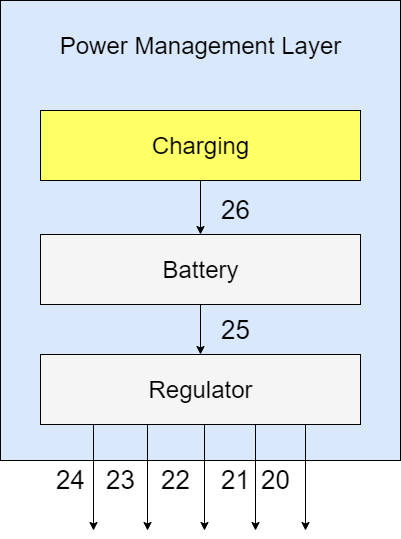
\includegraphics[width=0.60\textwidth]{images/PowerMgmtLayer_charging.drawio.png}
 \caption{Power Management Charging Subsystem diagram}
\end{figure}

\subsubsection{Assumptions}
%Any assumptions made in the definition of the subsystem should be listed and described. Pay particular attention to assumptions concerning interfaces and interactions with other layers.
The user has access to electricity and has the proper charging cable for the wristband.

\subsubsection{Responsibilities}
%Each of the responsibilities/features/functions/services of the subsystem as identified in the architectural summary must be expanded to more detailed responsibilities. These responsibilities form the basis for the identification of the finer-grained responsibilities of the layer's internal subsystems. Clearly describe what each subsystem does.
This subsystem is responsible for charging the wristband's battery. It must be able to charge the wristband within a reasonable time frame. It will take a USB-c cable that can be plugged into a USB outlet. 

\subsubsection{Subsystem Interfaces}
%Each of the inputs and outputs for the subsystem are defined here. Create a table with an entry for each labelled interface that connects to this subsystem. For each entry, describe any incoming and outgoing data elements will pass through this interface.

\begin{table}[H]
\caption{Charging Interfaces}
\begin{center}
\begin{tabular}{|l|l|l|l|}
    \hline
    ID & Description & Input & Output \\ \hline
    26 & Charging to battery & N/A & Voltage \\ \hline
\end{tabular}
\end{center}
\end{table}

\subsection{Battery}

\begin{figure}[h!]
	\centering
 	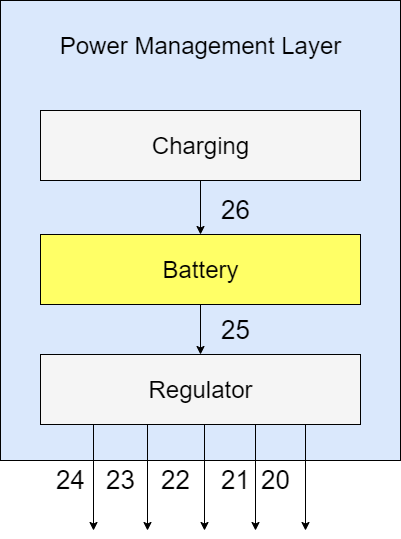
\includegraphics[width=0.60\textwidth]{images/PowerMgmtLayer_battery.drawio.png}
 \caption{Power Management Battery Subsystem diagram}
\end{figure}

\subsubsection{Assumptions}
%Any assumptions made in the definition of the subsystem should be listed and described. Pay particular attention to assumptions concerning interfaces and interactions with other layers.
The user has access to electricity to charge the battery. The battery is working properly and not damaged. 

\subsubsection{Responsibilities}
%Each of the responsibilities/features/functions/services of the subsystem as identified in the architectural summary must be expanded to more detailed responsibilities. These responsibilities form the basis for the identification of the finer-grained responsibilities of the layer's internal subsystems. Clearly describe what each subsystem does.
This subsystem is responsible for powering the all the wristband components. It must be strong enough to power all the wristband components. The battery must be long lasting to prevent the user from having to charge it constantly. 

\subsubsection{Subsystem Interfaces}

\begin{table}[H]
\caption{Battery Interfaces}
\begin{center}
\begin{tabular}{|l|l|l|l|}
    \hline
    ID & Description & Input & Output \\ \hline
    25 & Battery to Regulator  & Voltage  & Power (W)  \\ \hline
\end{tabular}
\end{center}
\end{table}

\subsection{Regulator}

\begin{figure}[h!]
	\centering
 	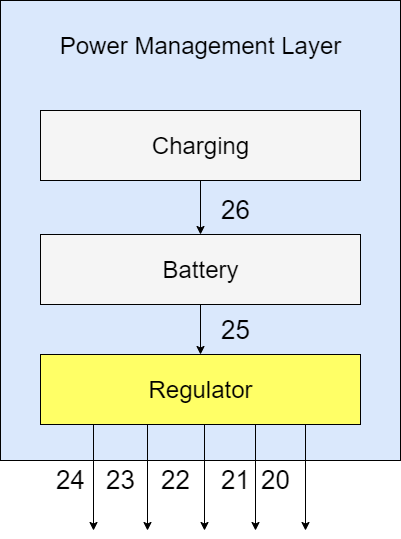
\includegraphics[width=0.60\textwidth]{images/PowerMgmtLayer_regulator.drawio.png}
 \caption{Power Management Regulator Subsystem diagram}
\end{figure}

\subsubsection{Assumptions}
%Any assumptions made in the definition of the subsystem should be listed and described. Pay particular attention to assumptions concerning interfaces and interactions with other layers.
The wristband is properly charged and working. The wristband is not damaged or malfunctioning. 

\subsubsection{Responsibilities}
%Each of the responsibilities/features/functions/services of the subsystem as identified in the architectural summary must be expanded to more detailed responsibilities. These responsibilities form the basis for the identification of the finer-grained responsibilities of the layer's internal subsystems. Clearly describe what each subsystem does.
This subsystem is responsible for regulating the power coming from the battery to the other wristband components. It must delegate enough power to each component so the wristband can function properly. It must not drain the battery too fast.

\subsubsection{Subsystem Interfaces}

\begin{table}[H]
\caption{Regulator interfaces}
\begin{center}
\begin{tabular}{|l|l|l|l|}
    \hline
    ID & Description & Inputs & Outputs \\ \hline
    24 & Power to Bluetooth Module & Power (W) & Power (W) \\ \hline
    23 & Power to Micro-Controller & Power (W) & Power (W) \\ \hline
    22 & Power to Vibration Module & Power (W) & Power (W) \\ \hline
    21 & Power to Audio Sensor & Power (W) & Power (W) \\ \hline
    20 & Power to LED lights & Power (W) & Power (W) \\ \hline
    % I think I am supposed to put all the wristband components here
\end{tabular}
\end{center}
\end{table}
